
Weit hinten, hinter den Wortbergen, fern der Länder Vokalien und Konsonantien leben die Blindtexte. Abgeschieden wohnen Sie in Buchstabhausen an der Küste des Semantik, eines gro"sen Sprachozeans. Ein kleines Bächlein namens Duden flie"st durch ihren Ort und versorgt sie mit den nötigen Regelialien. Es ist ein paradiesmatisches Land, in dem einem gebratene Satzteile in den Mund fliegen. Nicht einmal von der allmächtigen Interpunktion werden die Blindtexte beherrscht – ein geradezu unorthographisches Leben.

\section{Überschrift 2 (Abschnittsüberschrift)}

Eines Tages aber beschloss eine kleine Zeile Blindtext, ihr Name war Lorem Ipsum, hinaus zu gehen in die weite Grammatik. Der gro"se Oxmox riet ihr davon ab, da es dort wimmele von bösen Kommata, wilden Fragezeichen und hinterhältigen Semikoli, doch das Blindtextchen lie"s sich nicht beirren. Es packte seine sieben Versalien, schob sich sein Initial in den Gürtel und machte sich auf den Weg.\\
\\
Als es die ersten Hügel des Kursivgebirges erklommen hatte, warf es einen letzten Blick zurück auf die Skyline seiner Heimatstadt Buchstabhausen, die Headline von Alphabetdorf und die Subline seiner eigenen Stra"se, der Zeilengasse. Wehmütig lief ihm eine rethorische Frage über die Wange, dann setzte es seinen Weg fort. Unterwegs traf es eine Copy.

\subsection{Überschrift 3 (Unterabschnittsüberschrift)}

Die Copy warnte das Blindtextchen, da, wo sie herkäme wäre sie zigmal umgeschrieben worden und alles, was von ihrem Ursprung noch übrig wäre, sei das Wort "und" und das Blindtextchen solle umkehren und wieder in sein eigenes, sicheres Land zurückkehren. Doch alles Gutzureden konnte es nicht überzeugen und so dauerte es nicht lange, bis ihm ein paar heimtückische Werbetexter auflauerten, es mit Longe und Parole betrunken machten und es dann in ihre Agentur schleppten, wo sie es für ihre Projekte wieder und wieder missbrauchten.

\subsubsection{Überschrift 4 (Unterunterabschnittsüberschrift)}

Und wenn es nicht umgeschrieben wurde, dann benutzen Sie es immernoch. Weit hinten, hinter den Wortbergen, fern der Länder Vokalien und Konsonantien leben die Blindtexte. Abgeschieden wohnen Sie in Buchstabhausen an der Küste des Semantik, eines gro"sen Sprachozeans. Ein kleines Bächlein namens Duden flie"st durch ihren Ort und versorgt sie mit den nötigen Regelialien. Es ist ein paradiesmatisches Land, in dem einem gebratene Satzteile in den Mund fliegen. Nicht einmal von der allmächtigen Interpunktion werden die Blindtexte beherrscht – ein geradezu unorthographisches Leben. Eines Tages aber beschloss eine kleine Zeile Blindtext, ihr Name war Lorem Ipsum, hinaus zu gehen in die weite Grammatik. Der gro"se Oxmox riet ihr davon ab, da es dort wimmele von bösen Kommata, wilden Fragezeichen und hinterhältigen Semikoli, doch das Blindtextchen lie"s sich nicht beirren. Es packte seine sieben Versalien, schob sich sein Initial in den Gürtel und machte sich auf den Weg.\\
\\
Als es die ersten Hügel des Kursivgebirges erklommen hatte, warf es einen letzten Blick zurück auf die Skyline seiner Heimatstadt Buchstabhausen, die Headline von Alphabetdorf und die Subline seiner eigenen Stra"se, der Zeilengasse. Wehmütig lief ihm eine rethorische Frage über die Wange, dann setzte es seinen Weg fort. Unterwegs traf es eine Copy.

\normalsize

\chapter{Aufzählung, Abbildung und Tabelle im neuen Uni-Design}



%%%%%%%%%%%%%%%%%%%%%%%%%%%%%%%%
% Aufzählung                   %
%%%%%%%%%%%%%%%%%%%%%%%%%%%%%%%%

% Aufzählungen, sowohl numerisch mittels
%
%    enumerate
%
% als auch nicht-numerisch mittels
%
%    itemize
%
% können nach den Designvorlagen der Universität Konstanz
% erstellt werden. Außerdem sind auch verschiedene Ebenen möglich.

\section{Aufzählung}

Aufzählungen, sowohl numerisch als auch nicht-numerisch (item), können nach den Designvorlagen der Universität Konstanz erstellt werden. Au"serdem sind auch verschiedene Ebenen möglich.\\

\begin{enumerate}
\item Studienbereitschaft (Nummerische Aufzählung)

\begin{itemize}
\item Profil der Befragten (Absatzformat Aufzählungszeichen)
\item Anteil der Studierenden mit Migrationshintergrund
\item Anteil der Studierenden
\end{itemize}

\item Vor dem Studium und Studieneinstieg
\begin{itemize}
\item Studienentscheidung bzw. Studienwahl (Absatzformat Aufzählungszeichen)
\item Angebnote zur Studieneinstiegsphase
\item Schwierigkeiten in der Studieneinstiegsphase
\end{itemize}

\item Studium und Studienbedingungen
\begin{itemize}
\item Fachliche und didaktische Qualität der Lehre (Absatzformat Aufzählungszeichen)
\item Betreuung durch Lehrende
\item Forschungs- und Praxisbezug
\item Anforderungen und Schwierigkeiten im Studium
\end{itemize}

\item Noch mehr und tiefere Ebenen der Aufzählung

\begin{itemize}
\item Hier ist noch die erste Ebene (Absatzformat Aufzählungszeichen)
\item Ebenfalls noch die erste Ebene
\item Ebene 1
\begin{itemize}
\item Ab jetzt wird es eine ebene Tiefer (Absatzformat Aufzählungszeichen)
\item Ebene 2
\item Noch einmal Ebene 2
\item Und noch einmal Ebene \ldots
\item \ldots 2
\begin{itemize}
\item Und noch eine Ebene tiefer (Absatzformat Aufzählungszeichen)
\item Dies ist jetzt Ebene \ldots
\item \ldots 3
\end{itemize}
\end{itemize}
\end{itemize}

\item Prüfungssystem
\item Serviceangebote
\item Übergangsphasen

\end{enumerate}



%%%%%%%%%%%%%%%%%%%%%%%%%%%%%%%%
% Abbildung                    %
%%%%%%%%%%%%%%%%%%%%%%%%%%%%%%%%

% Auch Abbildungen können wie gewohnt mit der figure Umgebung
% im Corporate Design der Universität Konstanz erstellt werden.

\section{Abbildung}

Weit hinten, hinter den Wortbergen, fern der Länder Vokalien und Konsonantien leben die Blindtexte. Abgeschieden wohnen Sie in Buchstabhausen an der Küste des Semantik, eines gro"sen Sprachozeans. Ein kleines Bächlein namens Duden flie"st durch ihren Ort und versorgt sie mit den nötigen Regelialien. Es ist ein paradiesmatisches Land, in dem einem gebratene Satzteile in den Mund fliegen. Nicht einmal von der allmächtigen Interpunktion werden die Blindtexte beherrscht – ein geradezu unorthographisches Leben.\\
\\
Au"serdem zeigt Abbildung~\ref{fig:treppe} die Verteilung der Studenten und Studentinnen auf der Treppe an der Universität Konstanz.
\begin{figure}[H]
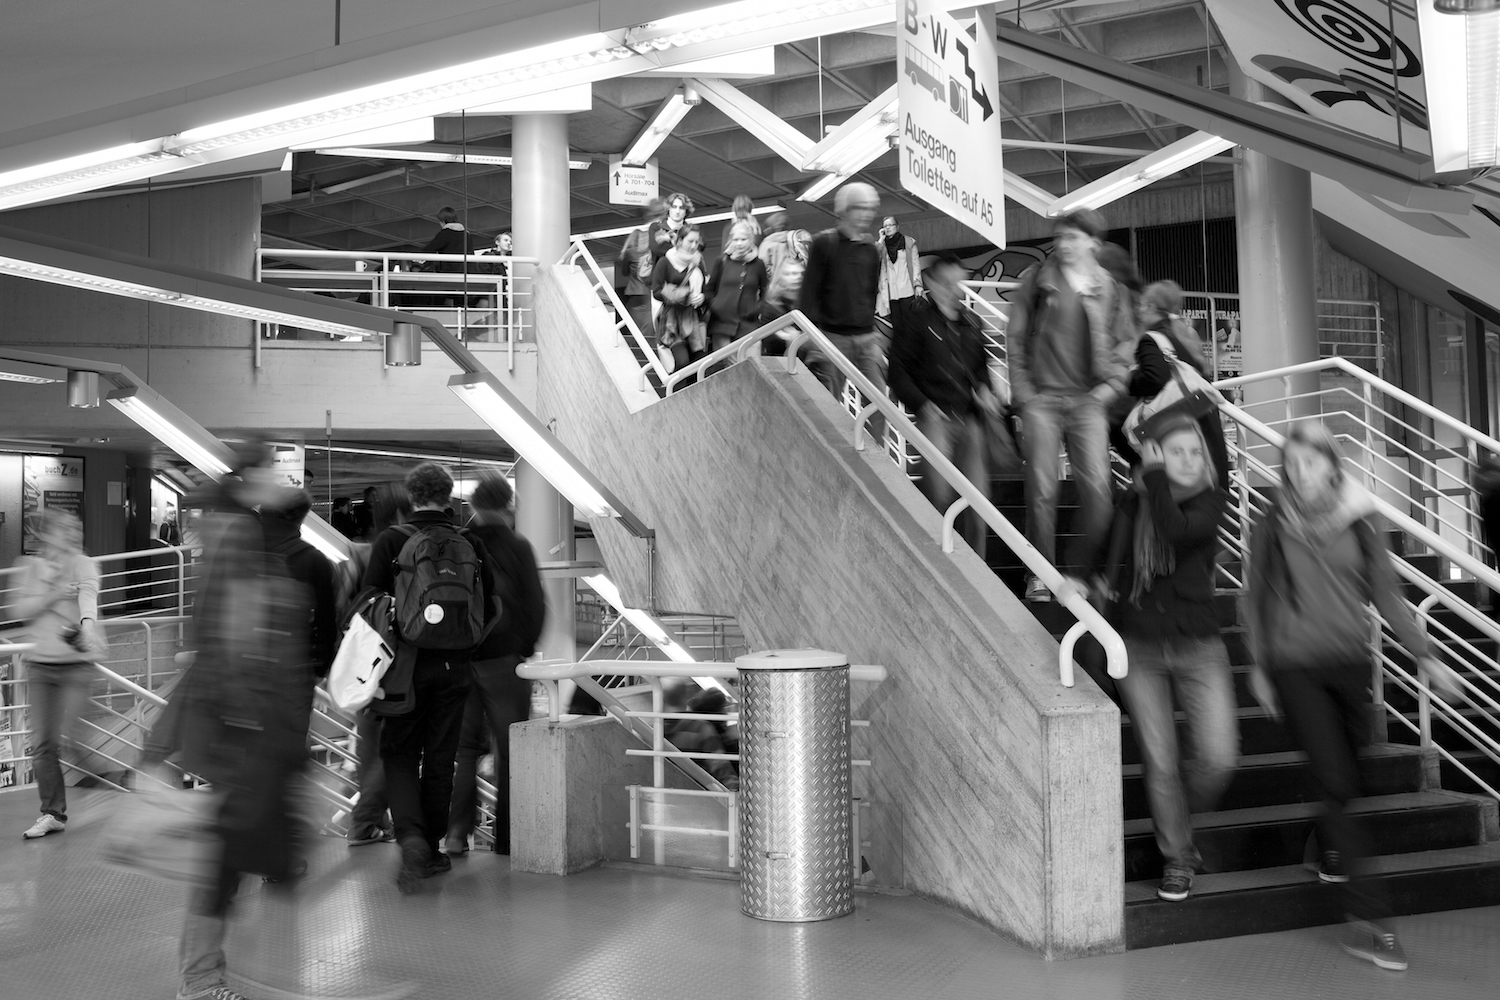
\includegraphics[width=\textwidth]{graphics/indoor_sw.png}
\caption{Verteilung der Studenten auf der Treppe}
\label{fig:treppe}
\end{figure}

\noindent Als es die ersten Hügel des Kursivgebirges erklommen hatte, warf es einen letzten Blick zurück auf die Skyline seiner Heimatstadt Buchstabhausen, die Headline von Alphabetdorf und die Subline seiner eigenen Stra"se, der Zeilengasse. Wehmütig lief ihm eine rethorische Frage über die Wange, dann setzte es seinen Weg fort. Unterwegs traf es eine Copy.



%%%%%%%%%%%%%%%%%%%%%%%%%%%%%%%%
% Tabelle                      %
%%%%%%%%%%%%%%%%%%%%%%%%%%%%%%%%

% Um eine Tabelle im Corporate Design der Universität Konstanz
% zu erstellen wird das Paket tabu verwendet. Dadurch ergeben
% sich auch kleine Unterschiede beim Erstellen von Tabellen.
%
% Als Umgebung muss tabu anstatt tabular verwendet werden:
%
%    \begin{tabu}
%
%        ...
%
%    \end{tabu}
%
% Die Spalten können direkt im Anschluss definiert werden.
%
%    { X[coef, align, type] X[coef, align, type] ... }
%
%    - coef skaliert die Spalten, sollten es mehrere sein
%    - align ist entweder r, l, c oder j
%    - type ist entweder p (Standard), m oder b
%    - Vertikale Linien können mittels | zwischen den Spalten
%      gezeichnet werden. Dies sollte aus ästehtischen Gründen
%      jedoch wenn möglich vermieden werden.
%
% Danach können wie aus der tabular Umgebung gewohnt die
% Zeilen definiert werden. Die Spalte wird mit % gewechselt und
% ein Zeilenumbruch kann mit \\ eingeleitet werden.
%
% Möchte man eine horizontale Linie zeichnen, so können nach
% dem Corporate Design der Universität Konstanz entweder
%
%    \unitoprule
%
% für eine durchgezogene (dicke) Linie in seeblau oder
%
%    \unimidrule
%
% eine gestrichelte durchgezogene Linie in seeblau gezeichnet
% werden.
%
% Da die tabu Umgebung sehr mächtig ist, können auch weitere
% Varianten gezeichnet werden. Dazu sein an die Paketdokumentation
% verwiesen:
%
%    ftp://ftp.fu-berlin.de/tex/CTAN/macros/latex/contrib/tabu/tabu.pdf
%
% Ein ausführliches Beispiel folgt gleich weiter unten.
%
% Die Tabelle sollte in einer table Umgebung eingebunden werden, damit
% sie im Tabellenverzeichnis erscheint. Außerdem kann noch eine Tabellen-
% überschrift hinzugefügt werden.

\section{Tabelle}

Die Copy warnte das Blindtextchen, da, wo sie herkäme wäre sie zigmal umgeschrieben worden und alles, was von ihrem Ursprung noch übrig wäre, sei das Wort "und" und das Blindtextchen solle umkehren und wieder in sein eigenes, sicheres Land zurückkehren. Doch alles Gutzureden konnte es nicht überzeugen und so dauerte es nicht lange, bis ihm ein paar heimtückische Werbetexter auflauerten, es mit Longe und Parole betrunken machten und es dann in ihre Agentur schleppten, wo sie es für ihre Projekte wieder und wieder missbrauchten.\\
\\
Auch Tabellen können nun im neuen Corporate Design der Universität Konstanz erstellt werden. Erfahren Sie mehr in der \texttt{.tex} Datei. Das Ergebnis können Sie in der Tabelle~\ref{tbl:Uni} bestaunen.

\begin{table}
\caption{Universitätsstatistik}
\label{tbl:Uni}
\selectfontsize{10pt}
\begin{tabu} {X[l]X[r]X[r]X[r]X[r]X[r]}
\unitoprule \\
\textbf{Wintersemester} & \textbf{2009/10} & \textbf{2010/11} & \textbf{2011/12} & \textbf{2012/13} & \textbf{2013/14} \\
\unitoprule \\
Mathematik & 456 & 428 & 526 & 542 & 529 \\
\unimidrule \\
Informatik & 266 & 308 & \ldots \\
\unimidrule \\
\ldots \\
\unimidrule \\
 \\
\unimidrule \\
 \\
\unitoprule \\
\textbf{Gesamt} & \textbf{9528} & \textbf{10081} & \textbf{10645} & \textbf{11337} & \textbf{11772} \\
\unitoprule \\
\end{tabu}
\end{table}

\normalsize

\chapter{Corporate Design Elemente}

Die vier Sättigungsstufen des \textbf{Seeblau} sind wie folgt definiert:

\begin{itemize}
\item \textcolor{seeblau100}{seeblau100}
\item \textcolor{seeblau65}{seeblau65}
\item \textcolor{seeblau35}{seeblau35}
\item \textcolor{seeblau20}{seeblau20}\\
\end{itemize}

\noindent Analog dazu die vier Sättigungsstufen der SW-Umsetzung:

\begin{itemize}
\item \textcolor{schwarz60}{schwarz60}
\item \textcolor{schwarz40}{schwarz40}
\item \textcolor{schwarz20}{schwarz20}
\item \textcolor{schwarz10}{schwarz10}\\
\end{itemize}



%%%%%%%%%%%%%%%%%%%%%%
% Schriftgröße       %
%%%%%%%%%%%%%%%%%%%%%%

% Da innerhalb einer Arbeit es meistens mehrere verschiedene Schriftgrößen
% gibt, steht hier das Makro
%
%     \selectfontsize
%
% zur Verfügung.
%
% Es kann jedoch auch die Latex internen Makros wie \Large, \small, o.ä.
% verwendet werden.
%
% Dieses Makro besitzt ein unbedingt notwendiges Argument und ein optionales
% Feld, indem Key-Value Pairs übergeben werden können.
%
%     \selectfontsize[<Key Value Pairs>]{<Schriftgröße>}
%
% Das Argument hat dabei folgende Bedeutung:
%
%   1. Argument:         Hier wird die neue Schriftgröße angegeben, die verwendet werden
%                        soll.
% Die weiteren Formatierungsoptionen werden alle innerhalb des optionalen Argumentes mittels
% Key-Value Pairs bestimmt.
%
% Dabei stehen folgende Optionen zur Verfügung:
%
%     baselineskip    Hier wird der baselineskip angegeben, welcher verwendet werden soll
%                     Mögliche Werte:
%                         0      Ist dieser 0, dann wird der baselinefaktor verwendet
%                         sonst
%                    Standardwert: 0
%
%     baselinefaktor Hier wird der Faktor angegeben, der verwendet wird, um den neuen
%                    baselineskip zu berechnen.
%                    Dieser wird nur benutzt, falls der baselineskip 0 beträgt.
%
%                        baselineskip = baselinefaktor * #1
%
%                    Standardwert: 12/10
%
%                    Da hier keine Fließkommazahl in der Dezimalschreibweise angegeben werden
%                    kann, müssen diese als Brüche repräsentiert werden, wie z.b. 12/10 anstatt
%                    1.2.
%
% Zurück zur Standardgröße gelangt man mit \normalsize

\noindent Neben den Standard in \LaTeX~verfügbaren Makros wie \texttt{\textbackslash large, \textbackslash LARGE, \textbackslash small, \ldots} zur Veränderung der Schriftgrö"se kann die Schriftgrö"se auch mittels des Makro

\begin{center}
\texttt{\textbackslash selectfontsize[baselinefaktor=<value>]\{<fontsize>\}}
\end{center}

\noindent oder

\begin{center}
\texttt{\textbackslash selectfontsize[baselinesize=<value>]\{<fontsize>\}}
\end{center}

\noindent verändert werden. Wird das optionale Argument weggelassen, wird automatisch der \texttt{baselinefaktor} 1.2 benutzt. Mehr dazu finden Sie auch in der Tex und in der Style Datei.\\
\\
Hier sind ein paar Beispiele:\\
\\
\selectfontsize{6pt} Ich bin eine sehr kleine Schriftgrö"se (6pt)\\
\selectfontsize{11pt} Ich bin sehr normal (11pt)\\
\selectfontsize{16pt} Ich bin schon grö"ser (16pt)\\
\selectfontsize{26pt} Ich bin ziemlich gro"s (26pt)\\
\selectfontsize{44pt} Ich bin riesig (44pt)%
%
% Zurück zur Standardgröße
\normalsize\\
\\
Zurück zur Standardgrö"se gelangt man mit

\begin{center}
\texttt{\textbackslash normalsize}
\end{center}

\newpage



\section{Markieren}

%%%%%%%%%%%%%%%%%%%%%%%%%
% CD Element: Markieren %
%%%%%%%%%%%%%%%%%%%%%%%%%

% Um einen Text mit Hilfe des Markieren Elements des Corporate Design hervorzuheben,
% steht das Makro
%
%     \markieren
%
% zur Verfügung.
%
% Dieses Makro besitzt vier unbedingt notwendige Argumente und ein optionales
% Feld, indem weitere EIgenschaften festgelegt werden könnnen..
%
%     \markieren[Optionen per Key-Value Pair]{<Zeile 1>}{<Zeile 2>}{<Zeile 3>}{<Zeile 4>}
%
% Die Argumente haben dabei folgende Bedeutung:
%
%   1. - 4. Argument:    Hier werden nun die eigentlichen Zeilen übergeben.
%
%                        Wichtig dabei ist es, dass die Aufteilung der Zeilen manuell erfolgen muss durch
%                        die Argumente, da nur somit sichergestellt werden kann, dass bspw. Treppeneffekte
%                        nicht auftreten und somit der Benutzer alle Freiheiten bei der Aufteilung besitzt.
%
%                        Sollten nicht alle Zeilen verwendet werden, dann müssen die hinteren Brackets
%                        leer gelassen werden, wie beispielsweise bei der Headline
%
% Die wichtigen Formatierungsoptionen werden alle innerhalb des optionalen Argumentes mittels
% Key-Value Pairs bestimmt.
%
% Dabei stehen folgende Optionen zur Verfügung:
%
%   align                Hier kann angegeben werden, ob das komplette Objekt
%                        links- oder rechtsbündig angeordent werden soll.
%
%                        Der Standardwert ist "left" und somit linksbündig.
%
%                        Für eine rechtsbündige Anordnung muss hier der Wert "right" hinterlegt werden.
%
%   vertical             Hier wird angegeben, ob der Inhalt der Zeilen zentriert werden soll oder
%                        überall an der gleichen Baseline ausgerichtet werden soll.
%
%                        Dies kann mittels der Wörter "center" und "base" eingestellt werden.
%                        Dabei ist "center" als Standardwert festgelegt.
%
%                        Der Unterschied besteht darin, dass bei Zeilen die Buchstaben mit einer Tiefe
%                        enthalten, wie g, p oder q, anders zentriert werden als welche ohne Buchstaben
%                        mit einer Tiefe.
%
%                        Da dies ein wenig Geschmackssache ist, werden hier beide Varianten zur Verfügung
%                        gestellt, wobei "center" primär verwendet werden soll, und "base" eher wenn
%                        Buchstaben mit einer Tiefe in den Zeilen enthalten sind.


Das \textbf{Markieren-Element} kann mit
\begin{center}
\texttt{\textbackslash markieren[<Optionen>]\{<Zeile 1>\}\{<Zeile 2>\}\{<Zeile 3>\}\{<Zeile 4>\}}
\end{center}
eingesetzt werden.\\
\\
Zudem stehen noch zwei optionale Argumente \texttt{align} und \texttt{vertical} zur Verfügung:\\
\begin{itemize}
\item Mittels \texttt{align} und den Werten \texttt{left} bzw. \texttt{right} kann die Ausrichtung des Markieren-Objektes festgelegt werden.
\item Mit der Option \texttt{vertical} und den Werten \texttt{center} und \texttt{base} kann die Ausrichtung innerhalb der Zeilen festgelegt werden.\\
\end{itemize}

\textsf{% Serienflose Schrift
\markieren{Ich bin}{eine}{Headline}{}\\
}%
\\
Hier sind noch mehr Markieren-Elemente in anderen Schriftgrö"sen:\\
\\
\textsf{% Serienflose Schrift
\begin{flushright}%
\selectfontsize{18pt}
\markieren[align=right]{\textbf{Ich bin}}{\textbf{eine}}{\textbf{Headline}}{}%
\end{flushright}%
\selectfontsize{24pt}
\markieren[vertical=base]{\textbf{Erste Zeile}}{\textbf{von einer}}{\textbf{vierzeiligen}}{\textbf{Headline}}%
}

\normalsize

\newpage



\section{Unterstreichen}

%%%%%%%%%%%%%%%%&%%%%%%%%%%%%%%
% CD Element: Unterstreichung %
%%%%%%%%%%%%%%%%%&%%%%%%%%%%%%%

% Um einen Text mit Hilfe des Unterstreichen Elements des Corporate Design hervorzuheben,
% steht das bereits bekannte Makro
%
%     \underline
%
% zur Verfügung, welches an die Anforderungen des Corporate Designs angepasst wurde.
%
% Dieses Makro besitzt ein notwendiges Argument
%
%     \underline{1. Argument}
%
% Das Argument hat folgende Bedeutung:
%
%   1. Argument: Hier wird der zu unterstreichende Text hinterlegt.
%
% Wichtig ist noch zu wissen, dass auch Textbrüche ohne Probleme durchgeführt werden können.
%
% Zudem können weitere Formatierungen, wie bold oder italic innerhalb des Argumentes angewendet
% werden.
%
% Die Dicke der unterstrichenen Linie passt sich dabei der aktuell verwendeten Textgröße an.

Das \textbf{Unterstreichen-Element} wird wie gewohnt mittels
\begin{center}
\texttt{\textbackslash underline\{<text>\}}
\end{center}
eingesetzt. Das Makro wurde dafür entsprechend angepasst.\\
\\
Möchte man einen fetten unterstrichenen Text haben, kann der zu unterstreichende Text einfach mittels \texttt{\textbackslash textbf\{\ldots\}} ergänzt werden:
\begin{center}
\texttt{\textbackslash underline\{\textbackslash textbf\{Ich bin der Anfang von einem Flie"stext mit Unterstreichen\}\}}
\end{center}
\underline{\textbf{Ich bin der Anfang von einem Flie"stext mit Unterstreichen}}\\
\\
Hier sind noch zwei weitere Beispiele:\\
\\
\underline{Ich bin eine Subline mit Unterstreichen}\\
\\
\underline{\textbf{Ich bin der Anfang von einem Flie"stext mit Unterstreichen}} und ich bin der weiterführende Flie"stext\ldots\\

\newpage



\section{Merken}

%%%%%%%%%%%%%%%%%%%%%%
% CD Element: Merken %
%%%%%%%%%%%%%%%%%%%%%%

% Um einen Text mit Hilfe des Merken Elements des Corporate Design hervorzuheben,
% steht das Makro
%
%     \merken
%
% zur Verfügung.
%
% Dieses Makro besitzt drei unbedingt notwendige Argumente
%
%     \merken{1. Argument}{2. Argument}{3. Argument}
%
% Die Argumente haben dabei folgende Bedeutung:
%
%   1. Argument: Hier wird die Breite des kompletten Objektes angegeben. Da das
%                Merken Objekt quadratisch ist, wird hier sowohl die Breite als auch
%                die Höhe angegeben.
%
%   2. Argument: Hier wird die Subline des Merken Elementes angegeben, die direkt unter der
%                Zeile mit dem X folgt (siehe auch Corporate Design Manual).
%
%   3. Argument: Hier wird der eigentliche Inhalt angegeben. Wichtig hierbei ist es,
%                dass dieser Inhalt an die untere Kante des Merken Elementes orientiert ist.
%                Somit entgegen der Subline (2. Argument), welche an die obere Kante abzüglich
%                der Zeile mit dem X orientiert ist.
%
% Hier folgt noch eine grafische Darstellung der Argumente:
%
%    |<------- 1. Argument ------->|
%
%    -------------------------------    -
%    |                           X |    ^
%    | Subline (2. Argument)       |    |
%    |                             |    1
%    |                             |    .
%    |                             |    A
%    |                             |    r
%    |                             |    g
%    |                             |    u
%    |                             |    m
%    |                             |    e
%    |                             |    n
%    |                             |    t
%    |                             |    |
%    | Inhalt (3. Argument)        |    v
%    -------------------------------    -
%
% Wichtig ist noch zu wissen, dass die Linienstärke und die Größe des X in der rechten oberen Ecke an die
% Höhe / Breite des Merken Elements dynamisch angepasst ist.

Das \textbf{Merken-Element} wird mit dem Makro
\begin{center}
\texttt{\textbackslash merken\{<Breite/Höhe>\}\{<Subline>\}\{<Inhalt>\}}
\end{center}
eingesetzt. Da das Merken-Element quadratisch ist, muss nur eine Grö"se angegeben werden. Ist keine Subline oder Inhalt erwünscht, sollen die dafür vorgesehenen Brackets einfach leer gelassen werden.\\
\\
\textsf{%
\merken{5cm}{}{\textbf{Hier steht etwas,} dass ich mir unbedingt merken oder das ich gesondert hervorheben möchte.}\\
}%
\\
Hier sind noch mehr Beispiele:\\
\\
\textsf{% Serienflose Schrift
\selectfontsize{28pt}%
\merken{7.5cm}{\selectfontsize{12pt}Bachelorstudiengang}{\textbf{Politik- und\\Verwaltungs-\\wissenschaft}}\selectfontsize{10pt}%
\hskip 1cm%
\merken{6cm}{}{\textbf{Kontakt}\\[0.5\baselineskip]Prof. Dr. Guido Burkard\\Universität Konstanz\\Fachbereich Physik\\Universitätsstra"se 10\\78464 Konstanz\\+49 7531 88-5256\\guido.burkard@uni-konstanz.de\\[0.5\baselineskip]\textbf{– uni-konstanz.de}}\\[1cm]%
\merken{4.5cm}{}{Die Universität Konstanz ist seit 2007 in allen drei Förderlinien der Exzellenzinitiative erfolgreich.}%
}
\newpage

\normalsize



\section{Block}

%%%%%%%%%%%%%%%%%%%%%%
% CD Element: Block  %
%%%%%%%%%%%%%%%%%%%%%%

% Mit dem Makro
%
%     \cdblock[Optionen per Key-Value Pair]{<Headline>}{<Spalte 1>}{<Spalte 2>}{<Spalte 3>}{<Spalte 4>}{<Spalte 5>}{<Spalte 6>}{<Spalte 7>}{<Spalte 8>}
%
% können Block-Elemente für z.B. wisschenschaftliche Inhalte erstellt werden.
%
% Dieses Makro besitzt 9 erforderliche Elemente, die bei jedem Aufruf angegeben werden müssen. Dabei
% ist es natürlich mögliche Argumente leer zu lassen, falls man diese nicht benötigt. Dies hat jedoch
% keinen Einfluss auf die Anzahl an Spalten. Diese müssen separat im Optionenargument angegeben werden
% mittels des Schlüssels columnnum (siehe weiter unten).
%
% Die Argumente haben dabei folgende Bedeutung:
%
%   1. Argument: Inhalt der Headline
%   2. Argument: Inhalt der 1. Spalte
%   3. Argument: Inhalt der 2. Spalte
%   4. Argument: Inhalt der 3. Spalte
%   5. Argument: Inhalt der 4. Spalte
%   6. Argument: Inhalt der 5. Spalte
%   7. Argument: Inhalt der 6. Spalte
%   8. Argument: Inhalt der 7. Spalte
%   9. Argument: Inhalt der 8. Spalte
%
%
% Die wichtigen Formatierungsoptionen werden diesmal alle innerhalb des optionalen Argumentes mittels
% Key-Value Pairs bestimmt.
%
% Dabei stehen folgende Optionen zur Verfügung:
%
%     thick          Hier wird die Dicke der Linie bestimmt.
%                    Die Pfeile werden generell mit der doppelten Dicke gezeichnet!
%                    Standardwert: \boxlinewidth
%
%     color          Hier wird die Farbe der Linie angegeben
%                    Es sollten nur die folgenden Farben benutzt werden:
%                        seeblau100
%                        seeblau65
%                        seeblau35
%                        seeblau20
%                        black
%                        schwarz60
%                        schwarz40
%                        schwarz20
%                        schwarz10
%                    Standardwert: seeblau100
%
%     width          Hier wird die Breite des Blocks angegeben
%                    Standardwert: \paperwidth
%
%     columnnum      Hier werden die Anzahl an Spalten definiert
%                    Standardwert: 4
%
%     headlinesep    Hier wird der Abstand zwischen der Headline und den Spalten angegeben
%                    Standardwert: Aktuelle Schriftgröße
%
%     columnspace    Hier wird der Abstand zwischen den Spalten angegeben
%                    Standardwert: Doppelte Schriftgröße
%
%     block          Hier kann angegeben werden, ob man einen Rahmen um diesen Block haben möchte
%                    Mögliche Werte: true, false
%                    Standardwert: false
%
%     inner          Hier kann angegeben werden, ob zwischen den Spalten Trennlinien haben möchte
%                    Mögliche Werte:
%                        false    keine Trennlinien
%                        short    Trennlinien, die so lange sind, wie der längste Nachbar (entweder der
%                                 linke oder rechte Nachbar
%                        long     Trennlinien, die bis nach ganz unten gehen. Sie sind also so lang
%                                 wie die längste Spalte
%                    Standardwert: false
%
%     inner1,        Hier kann für jeden Zwischenraum der Spalte exakt angegeben werden, ob Trennlinien
%     inner2,        existieren sollen und falls ja, wie lang sie sein sollen. Diese Werte werden jedoch
%     inner3,        nur berücksichtigt, wenn inner=false ist. Ansonsten ist inner stärker.
%     inner4,        Mögliche Werte:
%     inner5,           false    keine Trennlinien
%     inner6,           short    Trennlinien, die so lange sind, wie der längste Nachbar (entweder der
%     inner7,                    linke oder rechte Nachbar
%                       long     Trennlinien, die bis nach ganz unten gehen. Sie sind also so lang
%                                wie die längste Spalte
%                    Standardwert: false
%
%     outerleft,     Hier kann angegeben werden, ob links (rechts) der ersten Spalte eine Trennlinie existieren soll.
%     outerright     Mögliche Werte
%                        false    keine Trennlinien
%                        short    Trennlinien, die so lange sind, wie der direkte Nachbar (bei outerleft die 1. Spalte
%                                 und bei outerright die letzte Spalte
%                        long     Trennlinien, die bis nach ganz unten gehen. Sie sind also so lang
%                                 wie die längste Spalte
%                        verylong Trennlinie geht von oben nach unten, sowie ein halber columnspace nach innen.
%                    Standardwert: false
%
%     outertop,      Hier kann angegeben werden, ob oberhalb (unterhalb) des Blocks eine Trennlinie, oder ein Pfeil existieren soll.
%     outerbottom    Mögliche Werte
%                        false    keine Trennlinien
%                        long     Trennlinien, die von links nach rechts geht
%                        verylong Trennlinie, die von links nach rechts geht, sowie ein halber columnspace nach oben (unten).
%                        arrow    Pfeil, der aus der Trenlinie verylong besteht und in der Mitte einen Pfeil nach oben (unten)
%                                 besitzt.
%                    Standardwert: false
%
%     arrowtop1left, Hier kann angegeben werden, ob zwei Spalten oberhalb des Blocks mittels eines Doppelpfeils verbunden werden
%     arrowtop1right sollen. Da es maximal 8 Spalten sind, können auch nur maximal 4 Paare bestimmt werden.
%     arrowtop2left  Ein Paar besteht somit aus einer linken und einer rechten Spalte.
%     arrowtop2right Mögliche Werte:
%     arrowtop3left      0   Keine Auswahl
%     arrowtop3right     1-8 Auswahl einer Spalte von 1 bis 8
%     arrowtop4left  Standardwert: 0
%     arrowtop4right Sollte der linke Wert nicht kleiner als der rechte Wert sein, so werden keine Pfeile gezeichnet. Das gleiche
%                    gilt für Werte, die außerhalb des Bereichs liegen.
%
%
% Wichtig ist noch zu wissen, wie die Breite letztendlich berechnet wird:
% Da es auch links und rechts der Spalten Trennlinien oder Pfeile geben kann, ist links der 1. und rechts der
% letzten Spalte ebenfalls ein columnspace vorgesehen.
% Somit wird die Spaltenbreite wie folgt berechnet
%
%     blockcolumnwidth = (width - (columnspace * (columnnum + 1))) / columnnum
%

Das \textbf{Block-Element} welches vor allem auf Plakaten vorkommt, kann mit dem Makro
\begin{center}
\texttt{\textbackslash cdblock[<Optionen>]\{<Headline>\}\{<Spalte 1>\}\ldots\{<Spalte 8>\}}
\end{center}
eingesetzt werden. Die ganzen Optionen können in der Tex und in der Style Datei nachgelesen werden.\\
\\
Die Abbildungen~\ref{fig:block1},~\ref{fig:block2} und~\ref{fig:block3} zeigen drei Beispiele von Block Elementen im Corporate Design der Universität Konstanz.

\begin{sffamily} % serifenlose Schrift
\begin{figure}[H]
\cdblock[width=\textwidth-1cm, columnnum=4, columnspace=1cm, outerbottom=arrow, outertop=verylong, inner=long]{}{\textcolor{seeblau100}{\textbf{Spalte 1}}\\[\baselineskip]Dies ist die erste Spalte und hier kann eigentlich so alles mögliche stehen.}{\textcolor{seeblau100}{\textbf{Spalte 2}}\\[\baselineskip]Dies ist die zweite Spalte und hier kann auch wieder eine ganze Menge stehen}{\textcolor{seeblau100}{\textbf{Spalte 3}}\\[\baselineskip]Auch hier kann das ein oder andere wichtige stehen, oder sogar sehr wichtiges}{\textcolor{seeblau100}{\textbf{Spalte 4}}\\[\baselineskip]Und auch in der vierten Spalte findet man sicherlich einiges}{}{}{}{}%
\caption{Ein Block Element im Corporate Design}
\label{fig:block1}
\end{figure}

\begin{figure}[H]
\cdblock[width=\textwidth-1cm, columnnum=1, columnspace=1cm, outerleft=verylong, outerright=verylong]{\selectfontsize{18pt}\textcolor{seeblau100}{\textbf{Beweis}}}{Dieses Block-Element kann natürlich für Beweise und Beispiele sehr gut eingesetzt werden, da es im Corporate Design der Universität Konstanz ist.}{}{}{}{}{}{}{}\\[2\baselineskip]%
\caption{Ein weiteres Block Element im Corporate Design}
\label{fig:block2}
\end{figure}

\begin{figure}[H]
\cdblock[width=\textwidth-1cm, columnnum=1, columnspace=1cm, block=true]{\selectfontsize{18pt}\textcolor{seeblau100}{\textbf{Beispiel}}}{Dieses Beispiel hat einen kompletten Rahmen}{}{}{}{}{}{}{}%
\caption{Und noch ein Block Element im Corporate Design}
\label{fig:block3}
\end{figure}
\end{sffamily}

\normalsize
\newpage



\section{Pfeile und Linien}

%%%%%%%%%%%%%%%%%%%%%%%%%%%%%%%%%%%%%%%%%%%%%%
% CD Element: Linie (mit optionalen Pfeilen) %
%%%%%%%%%%%%%%%%%%%%%%%%%%%%%%%%%%%%%%%%%%%%%%

% Mit dem Makro
%
%     \cdline[Optionen per Key-Value Pair]{<Länge der Linie>}
%
% kann eine Linie mit einer bestimmten Länge erstellt werden.
%
% Dieses Makro besitzt 1 erforderliches Element, welches bei jedem Aufruf mit angegeben
% werden muss.
%
% Das Argument hat dabei folgende Bedeutung.
%
%   1. Argument: Länge der erzeugten Linie
%
%
% Die wichtigen Formatierungsoptionen werden alle innerhalb des optionalen Argumentes mittels
% Key-Value Pairs bestimmt.
%
% Dabei stehen folgende Optionen zur Verfügung:
%
%     thick          Hier wird die Dicke der Linie bestimmt
%                    Standardwert: \boxlinewidth
%
%     mode           Hier wird angegeben, ob die Linie horizontal oder vertikal ausgerichtet werden soll
%                    Mögliche Werte
%                        horizontal
%                        vertical
%                    Standardwert: horizontal
%
%     color          Hier wird die Farbe der Linie angegeben
%                    Es sollten nur die folgenden Farben benutzt werden:
%                        seeblau100
%                        seeblau65
%                        seeblau35
%                        seeblau20
%                        black
%                        schwarz60
%                        schwarz40
%                        schwarz20
%                        schwarz10
%                    Standardwert: seeblau100
%
%     arrowleft      Hier wird angegeben, die Linie am linken (vertical: oberen) Ende mit einem Pfeil enden soll
%                    Mögliche Werte:
%                        true
%                        false
%                    Standardwert: false
%
%     arrowright     Hier wird angegeben, die Linie am rechten (vertical: unteren) Ende mit einem Pfeil enden soll
%                    Mögliche Werte:
%                        true
%                        false
%                    Standardwert: false


Die \textbf{Linien-Elemente} welche vor allem auf Plakaten vorkommen, können mit dem Makro
\begin{center}
\texttt{\textbackslash cdline[<Optionen>]\{<Länge>\}}
\end{center}
eingesetzt werden.\\
\\
Mit den Optionen, welche Sie in der Tex und Style Datei finden, kann die Linienstärke, Ausrichtung, Farbe und die Pfeile angepasst werden.\\
\\
In den Abbildungen~\ref{fig:pfeil} und~\ref{fig:linie} finden Sie zwei Beispiele wie Pfeile oder Linien einfach im Uni-Design erstellt werden können.

\begin{sffamily} % serifenlose Schrift
\begin{figure}[H]
\centering\cdline[thick=8pt, arrowleft=true, arrowright=true]{10cm}\\
\caption{Ein dicker Pfeil im Corporate Design der Universität Konstanz}
\label{fig:pfeil}
\end{figure}

\begin{figure}[H]
\cdline[color=seeblau20, thick=8pt, mode=vertical]{1cm} \hskip 0.8cm \cdline[color=seeblau35, thick=8pt, mode=vertical]{1.5cm} \hskip 0.8cm \cdline[color=seeblau65, thick=8pt, mode=vertical]{2cm} \hskip 0.8cm \cdline[thick=8pt, mode=vertical]{2.5cm} \hskip 0.8cm \cdline[color=seeblau65, thick=8pt, mode=vertical]{2cm} \hskip 0.8cm \cdline[color=seeblau35, thick=8pt, mode=vertical]{1.5cm} \hskip 0.8cm \cdline[color=seeblau20, thick=8pt, mode=vertical]{1cm} \hskip 0.8cm \cdline[color=schwarz10, thick=8pt, mode=vertical]{1cm} \hskip 0.8cm \cdline[color=schwarz20, thick=8pt, mode=vertical]{1.5cm} \hskip 0.8cm \cdline[color=schwarz40, thick=8pt, mode=vertical]{2cm} \hskip 1cm \cdline[color=schwarz60, thick=8pt, mode=vertical]{2.5cm} \hskip 0.8cm \cdline[color=schwarz40, thick=8pt, mode=vertical]{2cm} \hskip 0.8cm \cdline[color=schwarz20, thick=8pt, mode=vertical]{1.5cm} \hskip 0.8cm \cdline[color=schwarz10, thick=8pt, mode=vertical]{1cm}%
\caption{Viele unterschiedlichen Linien in den Farben des Corporate Design}
\label{fig:linie}
\end{figure}
\end{sffamily}

\normalsize
\newpage



\section{Klammern}

%%%%%%%%%%%%%%%%%%%%%%%%%%%%%%%%%%%%%%%%%%%%%%%%
% CD Element: Klammer (mit optionalen Pfeilen) %
%%%%%%%%%%%%%%%%%%%%%%%%%%%%%%%%%%%%%%%%%%%%%%%%

% Mit dem Makro
%
%     \cdbracket[Optionen per Key-Value Pair]{<Breite des Klammer>}{<Höhe des Klammer>}
%
% kann eine Klammer mit einer bestimmten Breite und Höhe gezeichnet werden.
%
% Dieses Makro besitzt 2 erforderliche Elemente, welche bei jedem Aufruf mit angegeben
% werden müssen.
%
% Die Argumente haben dabei folgende Bedeutung.
%
%   1. Argument: Breite der erzeugten Klammer
%   2. Argument: Höhe der erzeugten Klammer
%
%
% Die wichtigen Formatierungsoptionen werden alle innerhalb des optionalen Argumentes mittels
% Key-Value Pairs bestimmt.
%
% Dabei stehen folgende Optionen zur Verfügung:
%
%     thick          Hier wird die Dicke der Linien bestimmt
%                    Standardwert: \boxlinewidth
%
%     mode           Hier wird die Ausrichtung der Klammer angegeben
%                    Mögliche Werte
%                        left    linke Klammer
%                        top     obere Klammer
%                        right   rechte Klammer
%                        bottom  untere Klammer
%                    Standardwert: left
%
%     color          Hier wird die Farbe der Linie angegeben
%                    Es sollten nur die folgenden Farben benutzt werden:
%                        seeblau100
%                        seeblau65
%                        seeblau35
%                        seeblau20
%                        black
%                        schwarz60
%                        schwarz40
%                        schwarz20
%                        schwarz10
%                    Standardwert: seeblau100
%
%     arrowleft      Hier wird angegeben, ob die Klammer am linken (oberen) Ende mit einem Pfeil enden soll
%                    Mögliche Werte:
%                        true
%                        false
%                    Standardwert: false
%
%     arrowright     Hier wird angegeben, ob die Klammer am rechten (unteren) Ende mit einem Pfeil enden soll
%                    Mögliche Werte:
%                        true
%                        false
%                    Standardwert: false
%
%     arrowmiddle    Hier wird angegeben, ob die Klammer in der Mitte einen weiteren Pfeil besitzen soll der in die
%                    andere Richtung der Klammer zeigt (wie beim Makro \block mit der Optione arrow bei outerbottom / outertop)
%                    Mögliche Werte:
%                        true
%                        false
%                    Standardwert: false


Die \textbf{Klammer-Elemente} welche ebenfalls auf Plakaten verwendet werden, können mit dem Makro
\begin{center}
\texttt{\textbackslash cdbracket[<Optionen>]\{<Breite>\}\{<Höhe>\}}
\end{center}
eingesetzt werden.\\
\\
Mit den Optionen, welche Sie in der Tex und Style Datei finden, können wieder Formatierungen vorgenommen werden.\\
\\
In den Abbildungen~\ref{fig:klammer1} und~\ref{fig:klammer2} sehen Sie zwei verschiedene Klammern, mit und ohne Pfeile.

\begin{sffamily}% Serienflose Schrift
\begin{figure}[H]
\centering\cdbracket[thick=8pt, mode=bottom, arrowleft=true, arrowright=true, arrowmiddle=true]{10cm}{2cm}
\caption{Eine sehr multifunktionale Klammer}
\label{fig:klammer1}
\end{figure}

\begin{figure}[H]
\centering\cdbracket[mode=left]{2cm}{8cm}
\caption{Eine weitere multifunktionale Klammer}
\label{fig:klammer2}
\end{figure}
\end{sffamily}

\normalsize

\newpage

\chapter{Weitere Hinweise und Sonstiges}

Alle verwendeten Makros und Umgebeungen, die zur Erstellung von PDF-Dokumenten und Abschlussarbeiten benötigt werden, können aus dem Paket themeKonstanz geladen werden, dass sich in der Datei \texttt{themeKonstanz.sty} befindet.\\
\\
Möchte man dieses Dokument mit XeLaTeX anstatt LaTex kompilieren um die Systemschrift Arial zu verwenden, dann muss zusätzlich das Add-On Paket themeKonstanzXelatexAddOn, welches sich in der Datei themeKonstanzXelatexAddOn.sty befindet VOR dem eigentlichen Paket themeKonstanz geladen werden. XeLaTeX wird bereits in den meisten TeX-Distributionen mitgeliefert. Sollte es nicht mitgeliefert sein, kann es problemlos nachinstalliert
werden.\\
\\
Möchte man ein Style Add-On verwenden, das aus meiner Bachelorarbeit\footnote{Physischer Datenbankentwurf für ein NoSQL System anhand eines ER-Modells und gewichteter Transaktionen} aus dem Jahr 2015 stammt, so muss NACH dem Laden des Paketes themeKonstanz das zusätzliche Paket themeKonstanzStyleAddOn, welches sich in der Datei themeKonstanzStyleAddOn.sty befindet laden. Dabei werden die Überschriften der Kapitel, der Abschnitte, der Unterabschnitte und des Unterunterabschnittes geändert.\\
\\
Für das Erstellen der Elemente des Corporate Design werden einige
weitere Pakete benötigt. In der folgenden Liste sind die notwendigen
Pakete aufgelistet, die nicht überall standardmä"sig vorinstalliert sind:\\
\begin{itemize}
\item xcolor
\item textpos
\item xunicode
\item soul
\item tikz
\item ifthen
\item keycommand
\item calc
\item float
\item cmbright
\item fontspec
\item caption
\item chngcntr
\item tabu
\item fixltx2e (ab Tex-Version 2015 nicht mehr notwendig)
\item fancyhdr
\item titlesec \\
\end{itemize}
Zudem kann es sein, dass diese Pakete weitere Pakete voraussetzen. Diese müssen dann ebenfalls installiert werden. Der Compiler wird für diesen Fall die Pakete
anzeigen, welche zusätzlich noch benötigt werden.\\
\\
Des Weiteren ist es wichtig, dass alle Pakete, sowie ihre Tex-Distribution auf dem aktuellen Stand sind, um mögliche Probleme aus dem Weg zu gehen.\\
\\
Sollten Sie Probleme beim Kompilieren haben, können Sie dieses Dokument auch online, in Overleaf, unter \url{https://www.overleaf.com/6205861nhvynn} einsehen, bearbeiten und kompilieren.



%%%%%%%%%%%%%%%%%%%%%%%%%%%%%%%%
% Literaturverzeichnis         %
%%%%%%%%%%%%%%%%%%%%%%%%%%%%%%%%

% Zum Schluss kann noch das Literaturvzerzeichnis hinzugefügt
% werden.
%
% Damit es ebenfalls im Inhaltsverzeichnis gefunden werden kann,
% sollte das Literaturverzeichnis mit dem Makro
%
%    \addcontentsline{toc}{chapter}{Literaturverzeichnis}
%
% hinzugefügt werden.


\begin{thebibliography}{[MB91a]}
\addcontentsline{toc}{chapter}{Literaturverzeichnis}

\normalsize
\sffamily

\setlength{\itemsep}{6pt}

\bibitem[Cd15]{bib:corporateDesign}
Universität Konstanz: Corporate Design Manual.
Universtät Konstanz, (2015)

\end{thebibliography}
